% !Rnw weave = knitr
% The Data
\section{Analyzing All Data}
\label{sec:overall}
Here we analyze all of the data.

First we load the data and view a portion of it. Some more details.
\begin{knitrout}
\definecolor{shadecolor}{rgb}{1, 1, 1}\color{fgcolor}\begin{kframe}
\begin{alltt}
\hlfunctioncall{require}(useful)
\hlfunctioncall{load}(\hlstring{"C:/Users/Jared/week2/data/pakistan/pak.rdata"})
\hlfunctioncall{source}(\hlstring{"C:/Users/Jared/week2/R/distFuncs.r"})
\hlfunctioncall{corner}(pak, c = 15)
\end{alltt}
\begin{verbatim}
##   New_ID Age  Sex     Date Province District Tehsil        Village
## 1   1288  26 Male 29082010      KPK  Shangla Besham abaseen colony
## 2   1290  30 Male 29082010      KPK  Shangla Besham abaseen colony
## 3   1370  54 Male 28082010      KPK  Shangla Besham abaseen colony
## 4   1372  53 Male 28082010      KPK  Shangla Besham abaseen colony
## 5   1371  64 Male 28082010      KPK  Shangla Besham abaseen colony
##   Latitude Longitude Total Urban Rural
## 1    34.94     72.88  90.6     -  90.6
## 2    34.94     72.88  90.6     -  90.6
## 3    34.94     72.88  90.6     -  90.6
## 4    34.94     72.88  90.6     -  90.6
## 5    34.94     72.88  90.6     -  90.6
##                                 Accommodation StagnantWater
## 1 Collective centers (school/Public building)           Few
## 2                                 Host family           Few
## 3          On the site of the house (Damaged)           Few
## 4          On the site of the house (Damaged)          None
## 5          On the site of the house (Damaged)          None
\end{verbatim}
\end{kframe}
\end{knitrout}





Now we build a distribution for all the data and visualize it in Figure~\ref{fig:fullDist} with the code here:.
\begin{knitrout}
\definecolor{shadecolor}{rgb}{1, 1, 1}\color{fgcolor}\begin{kframe}
\begin{alltt}
ricePerc <- \hlfunctioncall{build.dist}(data = pak, lhs = \hlstring{"New_ID"}, group = \hlstring{"Province"}, question = \hlstring{"RiceLost"})
ricePerc$Size <- \hlstring{"All"}
\hlfunctioncall{ggplot}(ricePerc, \hlfunctioncall{aes}(x = RiceLost, y = Percent)) + \hlfunctioncall{geom_bar}(stat = \hlstring{"identity"}) + 
    \hlfunctioncall{facet_wrap}(~Province) + \hlfunctioncall{opts}(axis.text.x = \hlfunctioncall{theme_text}(angle = 90))
\end{alltt}
\end{kframe}
\end{knitrout}


\begin{figure}[!hbt]
\begin{knitrout}
\definecolor{shadecolor}{rgb}{1, 1, 1}\color{fgcolor}\begin{kframe}
\begin{alltt}
ricePerc <- \hlfunctioncall{build.dist}(data = pak, lhs = \hlstring{"New_ID"}, group = \hlstring{"Province"}, question = \hlstring{"RiceLost"})
ricePerc$Size <- \hlstring{"All"}
\hlfunctioncall{ggplot}(ricePerc, \hlfunctioncall{aes}(x = RiceLost, y = Percent)) + \hlfunctioncall{geom_bar}(stat = \hlstring{"identity"}) + 
    \hlfunctioncall{facet_wrap}(~Province) + \hlfunctioncall{opts}(axis.text.x = \hlfunctioncall{theme_text}(angle = 90))
\end{alltt}


{\ttfamily\noindent\textcolor{warningcolor}{\#\# Warning: 'opts' is deprecated.\\\#\# Use 'theme' instead.\\\#\# See help("Deprecated")}}

{\ttfamily\noindent\textcolor{warningcolor}{\#\# Warning: 'theme\_text' is deprecated.\\\#\# Use 'element\_text' instead.\\\#\# See help("Deprecated")}}\end{kframe}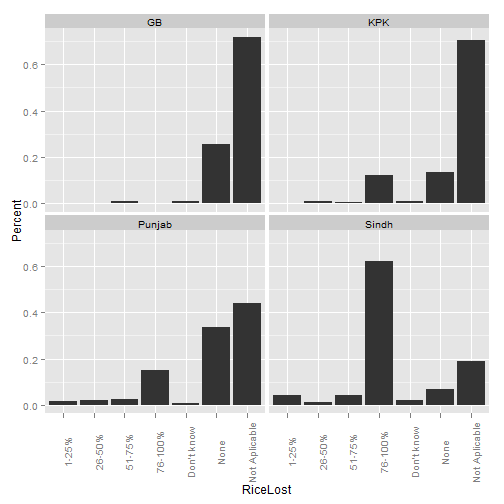
\includegraphics[width=.9\linewidth]{overall/figures/overallDistPlot} 
\end{knitrout}

\caption{Graphical view of the distribution of responses for all the data.\label{fig:fullDist}}
\end{figure}

In Section~\ref{sec:smallerDist} we analyze the distribution of responses for samples of fewer Tehsils.
